% Options for packages loaded elsewhere
\PassOptionsToPackage{unicode}{hyperref}
\PassOptionsToPackage{hyphens}{url}
%
\documentclass[
]{book}
\usepackage{amsmath,amssymb}
\usepackage{lmodern}
\usepackage{ifxetex,ifluatex}
\ifnum 0\ifxetex 1\fi\ifluatex 1\fi=0 % if pdftex
  \usepackage[T1]{fontenc}
  \usepackage[utf8]{inputenc}
  \usepackage{textcomp} % provide euro and other symbols
\else % if luatex or xetex
  \usepackage{unicode-math}
  \defaultfontfeatures{Scale=MatchLowercase}
  \defaultfontfeatures[\rmfamily]{Ligatures=TeX,Scale=1}
\fi
% Use upquote if available, for straight quotes in verbatim environments
\IfFileExists{upquote.sty}{\usepackage{upquote}}{}
\IfFileExists{microtype.sty}{% use microtype if available
  \usepackage[]{microtype}
  \UseMicrotypeSet[protrusion]{basicmath} % disable protrusion for tt fonts
}{}
\makeatletter
\@ifundefined{KOMAClassName}{% if non-KOMA class
  \IfFileExists{parskip.sty}{%
    \usepackage{parskip}
  }{% else
    \setlength{\parindent}{0pt}
    \setlength{\parskip}{6pt plus 2pt minus 1pt}}
}{% if KOMA class
  \KOMAoptions{parskip=half}}
\makeatother
\usepackage{xcolor}
\IfFileExists{xurl.sty}{\usepackage{xurl}}{} % add URL line breaks if available
\IfFileExists{bookmark.sty}{\usepackage{bookmark}}{\usepackage{hyperref}}
\hypersetup{
  hidelinks,
  pdfcreator={LaTeX via pandoc}}
\urlstyle{same} % disable monospaced font for URLs
\usepackage{color}
\usepackage{fancyvrb}
\newcommand{\VerbBar}{|}
\newcommand{\VERB}{\Verb[commandchars=\\\{\}]}
\DefineVerbatimEnvironment{Highlighting}{Verbatim}{commandchars=\\\{\}}
% Add ',fontsize=\small' for more characters per line
\usepackage{framed}
\definecolor{shadecolor}{RGB}{248,248,248}
\newenvironment{Shaded}{\begin{snugshade}}{\end{snugshade}}
\newcommand{\AlertTok}[1]{\textcolor[rgb]{0.94,0.16,0.16}{#1}}
\newcommand{\AnnotationTok}[1]{\textcolor[rgb]{0.56,0.35,0.01}{\textbf{\textit{#1}}}}
\newcommand{\AttributeTok}[1]{\textcolor[rgb]{0.77,0.63,0.00}{#1}}
\newcommand{\BaseNTok}[1]{\textcolor[rgb]{0.00,0.00,0.81}{#1}}
\newcommand{\BuiltInTok}[1]{#1}
\newcommand{\CharTok}[1]{\textcolor[rgb]{0.31,0.60,0.02}{#1}}
\newcommand{\CommentTok}[1]{\textcolor[rgb]{0.56,0.35,0.01}{\textit{#1}}}
\newcommand{\CommentVarTok}[1]{\textcolor[rgb]{0.56,0.35,0.01}{\textbf{\textit{#1}}}}
\newcommand{\ConstantTok}[1]{\textcolor[rgb]{0.00,0.00,0.00}{#1}}
\newcommand{\ControlFlowTok}[1]{\textcolor[rgb]{0.13,0.29,0.53}{\textbf{#1}}}
\newcommand{\DataTypeTok}[1]{\textcolor[rgb]{0.13,0.29,0.53}{#1}}
\newcommand{\DecValTok}[1]{\textcolor[rgb]{0.00,0.00,0.81}{#1}}
\newcommand{\DocumentationTok}[1]{\textcolor[rgb]{0.56,0.35,0.01}{\textbf{\textit{#1}}}}
\newcommand{\ErrorTok}[1]{\textcolor[rgb]{0.64,0.00,0.00}{\textbf{#1}}}
\newcommand{\ExtensionTok}[1]{#1}
\newcommand{\FloatTok}[1]{\textcolor[rgb]{0.00,0.00,0.81}{#1}}
\newcommand{\FunctionTok}[1]{\textcolor[rgb]{0.00,0.00,0.00}{#1}}
\newcommand{\ImportTok}[1]{#1}
\newcommand{\InformationTok}[1]{\textcolor[rgb]{0.56,0.35,0.01}{\textbf{\textit{#1}}}}
\newcommand{\KeywordTok}[1]{\textcolor[rgb]{0.13,0.29,0.53}{\textbf{#1}}}
\newcommand{\NormalTok}[1]{#1}
\newcommand{\OperatorTok}[1]{\textcolor[rgb]{0.81,0.36,0.00}{\textbf{#1}}}
\newcommand{\OtherTok}[1]{\textcolor[rgb]{0.56,0.35,0.01}{#1}}
\newcommand{\PreprocessorTok}[1]{\textcolor[rgb]{0.56,0.35,0.01}{\textit{#1}}}
\newcommand{\RegionMarkerTok}[1]{#1}
\newcommand{\SpecialCharTok}[1]{\textcolor[rgb]{0.00,0.00,0.00}{#1}}
\newcommand{\SpecialStringTok}[1]{\textcolor[rgb]{0.31,0.60,0.02}{#1}}
\newcommand{\StringTok}[1]{\textcolor[rgb]{0.31,0.60,0.02}{#1}}
\newcommand{\VariableTok}[1]{\textcolor[rgb]{0.00,0.00,0.00}{#1}}
\newcommand{\VerbatimStringTok}[1]{\textcolor[rgb]{0.31,0.60,0.02}{#1}}
\newcommand{\WarningTok}[1]{\textcolor[rgb]{0.56,0.35,0.01}{\textbf{\textit{#1}}}}
\usepackage{longtable,booktabs,array}
\usepackage{calc} % for calculating minipage widths
% Correct order of tables after \paragraph or \subparagraph
\usepackage{etoolbox}
\makeatletter
\patchcmd\longtable{\par}{\if@noskipsec\mbox{}\fi\par}{}{}
\makeatother
% Allow footnotes in longtable head/foot
\IfFileExists{footnotehyper.sty}{\usepackage{footnotehyper}}{\usepackage{footnote}}
\makesavenoteenv{longtable}
\usepackage{graphicx}
\makeatletter
\def\maxwidth{\ifdim\Gin@nat@width>\linewidth\linewidth\else\Gin@nat@width\fi}
\def\maxheight{\ifdim\Gin@nat@height>\textheight\textheight\else\Gin@nat@height\fi}
\makeatother
% Scale images if necessary, so that they will not overflow the page
% margins by default, and it is still possible to overwrite the defaults
% using explicit options in \includegraphics[width, height, ...]{}
\setkeys{Gin}{width=\maxwidth,height=\maxheight,keepaspectratio}
% Set default figure placement to htbp
\makeatletter
\def\fps@figure{htbp}
\makeatother
\setlength{\emergencystretch}{3em} % prevent overfull lines
\providecommand{\tightlist}{%
  \setlength{\itemsep}{0pt}\setlength{\parskip}{0pt}}
\setcounter{secnumdepth}{5}
\usepackage{booktabs}
\usepackage{amsthm}
\makeatletter
\def\thm@space@setup{%
  \thm@preskip=8pt plus 2pt minus 4pt
  \thm@postskip=\thm@preskip
}
\makeatother
\ifluatex
  \usepackage{selnolig}  % disable illegal ligatures
\fi
\usepackage[]{natbib}
\bibliographystyle{apalike}

\author{}
\date{\vspace{-2.5em}2021-03-16}

\begin{document}

{
\setcounter{tocdepth}{1}
\tableofcontents
}
\hypertarget{preface}{%
\chapter*{Preface}\label{preface}}
\addcontentsline{toc}{chapter}{Preface}

\hypertarget{intro}{%
\chapter{Introduction}\label{intro}}

This is the introduction for this project. Before that, I would like to introduce some terms involved in this project.

\begin{itemize}
\item
  R language : R is a language and environment for statistical computing and graphics which can be extended easily via packages and provide an Open Source route to participation in statistical methodology. It is available as Free Software under the term of the Free Software Foundation's GNU General Public License\citep{gnu}.
\item
  R Studio : It is an integrated development environment (IDE) for R. It includes a console, syntax-highlighting editor that supports direct code execution, as well as tools for plotting, history, debugging and workspace management.
\item
  R Packages : They are collections of functions and data sets developed by the community. They increase the power of R by improving existing base R functionalities, or by adding new ones.
\item
  CRAN : It is a network of ftp and web servers around the world that store identical, up-to-date, versions of code and documentation for R.
\item
  CRAN mirror : It is a website containing differently located servers, which aims to facilitate people from different regions and countries to access CRAN more smoothly and quickly. And each server is called a mirror.
\item
  API : It is the abbreviation of Application Programming Interface, which is a software intermediary that allows two applications to talk to each other.
\end{itemize}

\hypertarget{rtrends}{%
\section{rtrends}\label{rtrends}}

And then we come to the related literatures, which are as followed:

\begin{itemize}
\tightlist
\item
  \href{https://cran.r-project.org/web/packages/rtrends/rtrends.pdf}{\texttt{rtrends}}
  This is a package used for simple analysis of download logs from the CRAN RStudio Mirror, which contains one dataset and five functions. It's mainly functions are:
\end{itemize}

\begin{enumerate}
\def\labelenumi{(\arabic{enumi})}
\tightlist
\item
  abstract all CRAN download logs for a specific date
\item
  abstract CRAN download logs for a specific package
\item
  abstract CRAN download logs for a several package in a range of dates
\item
  merge CRAN download logs with county names
\item
  provide sample formatted CRAN logs
\end{enumerate}

\begin{itemize}
\item
  \href{https://github.com/lindbrook/packageRank}{\texttt{packageRank}}.
  It is also a package that relies on package \texttt{cranlog} and extends its functionality.It can publish the total download logs from CRAN with a more user-friendly interface and providing generic R \texttt{plot()} methods to make visualization easy. Also, many package creators are very concerned about the popularity of their packages, and this package \texttt{packageRank} can show the percentage of packages with less downloads. Furthermore, when we count the download logs, the exact thing we want is the number of times the package has been completely downloaded. In fact, we often encounter some wrongly sized download records, that is to say, users only download a part of the normal sized package. One is called ``medium'', the other is ``small'', which exists either as a part of pair with a full download or one of triplet with a ``medium'' and a full downloads. In order to deal with this, the creator filters the ``small'' entries that are less 1000 bytes and use triplet-specific filter to do with the ``medium'' entries.
\item
  \href{https://github.com/r-hub/cranlogs}{\texttt{cranlogs}} - to download the summary download data.
  It is a R package used to publish the total download logs from CRAN mirror in last day, last week or even a specific time range, for one package or several packages. And it can used to figure out the top downloaded packages in a time.
\item
  \href{https://github.com/tylermorganwall/adjustedcranlogs}{\texttt{adjustedcranlogs}}.
  We already know that the main function of \texttt{cranlogs} is to show the total number of download logs, but in practice, so the statistics of that will face the following problems: including the number of shared download logs, the same user downloads the same package again for some reason, and when a package is updated, the number of download logs will surge. Due to that, \texttt{adjustedcranlogs} is a wrapper around the \texttt{cranlogs} package that removes these three types of download logs. Therefore, using the data processed by this package to plot, we will find that the fluctuation of the download logs will be smaller.
\item
  \href{https://github.com/arunsrinivasan/cran.stats}{\texttt{cran.stats}}
  This package can also be used to get the total number of download logs first, but it is different from the previous package in that it gets seasonal data, such as annual, monthly and weekly. Besides, packages can have dependencies with each other, which means when a package is downloaded, its dependent package is also downloaded. But this will cause a problem, that is, when users download a package with its dependent package also downloaded, the download logs may not reflect the actual popularity of that dependent package. Therefore, another function of this package can solve this problem well by identifying and subtracting the downloads due to it's dependent packages. Also, there is one function used to plot direct downloads and downloads due to dependencies separately.
\item
  \href{https://github.com/GuangchuangYu/dlstats}{\texttt{dlstats}}
\item
  \href{https://github.com/r-hub/pkgsearch/}{\texttt{pkgsearch}}
  This is a package used to query packages in multiple dimensions. First, users can search by the usage of the package, and \texttt{pkgsearch} will return the results with popular packages before less frequently used ones. Or there is a \texttt{CRAN\ package\ search} addin in menu, with which users can search packages by clicking easily. And it can publish the version history of certain package or display the recent trending packages in detail. Besides, it can provide the latest releases or archivals. Moreover, the search server uses the stems of the words in the indexed metadata, and the search phrase. In this way, the deceleration result will not be affected by the grammar of spelling and tense, which increases the fault tolerance rate and become more user-friendly. At this point, there is also a functional extension, that is, the search engine prefers matching whole phrases over single words.This means that it will consider more about the meaning of the entire search term than match a word, which makes the results more accurate. For example, the search phrase ``permutation test'' will rank coin higher than testthat, even though testthat is a much better result for the single word ``test''. And it uses weighted scoring to show the ranking of the results, which includes reverse dependencies, matching degree of title and description and the number of downloads. Finally, it also provides ASCII folding for easy retrieval. In general, this is a comprehensive, practical and interesting search package.
\item
  \href{https://cran.r-project.org/web/packages/Visualize.CRAN.Downloads/vignettes/Visualize.CRAN.Downloads.html}{\texttt{Visualize.CRAN.Downloads}}
  This package provides a variety of methods and different types of presentation to visualize the downloads of packages, including static plots, interactive plots and comparison plot. These visualizations mainly focus on the single or comparative study of package downloads in a certain period of time. It includes the change of daily download volume with time, the change of cumulative total download volume, the fluctuation of average download volume and download volume within the standard deviation. In addition, it also provides many function options for splitting or combining figures to make visualization as comprehensive and flexible as possible.
\end{itemize}

\hypertarget{helpful-tips}{%
\section{Helpful tips}\label{helpful-tips}}

You can label chapter and section titles using \texttt{\{\#label\}} after them, e.g., we can reference Chapter \ref{intro}. If you do not manually label them, there will be automatic labels anyway, e.g., Chapter \ref{methods}.

Figures and tables with captions will be placed in \texttt{figure} and \texttt{table} environments, respectively.

\begin{Shaded}
\begin{Highlighting}[]
\FunctionTok{par}\NormalTok{(}\AttributeTok{mar =} \FunctionTok{c}\NormalTok{(}\DecValTok{4}\NormalTok{, }\DecValTok{4}\NormalTok{, .}\DecValTok{1}\NormalTok{, .}\DecValTok{1}\NormalTok{))}
\FunctionTok{plot}\NormalTok{(pressure, }\AttributeTok{type =} \StringTok{\textquotesingle{}b\textquotesingle{}}\NormalTok{, }\AttributeTok{pch =} \DecValTok{19}\NormalTok{)}
\end{Highlighting}
\end{Shaded}

\begin{figure}

{\centering 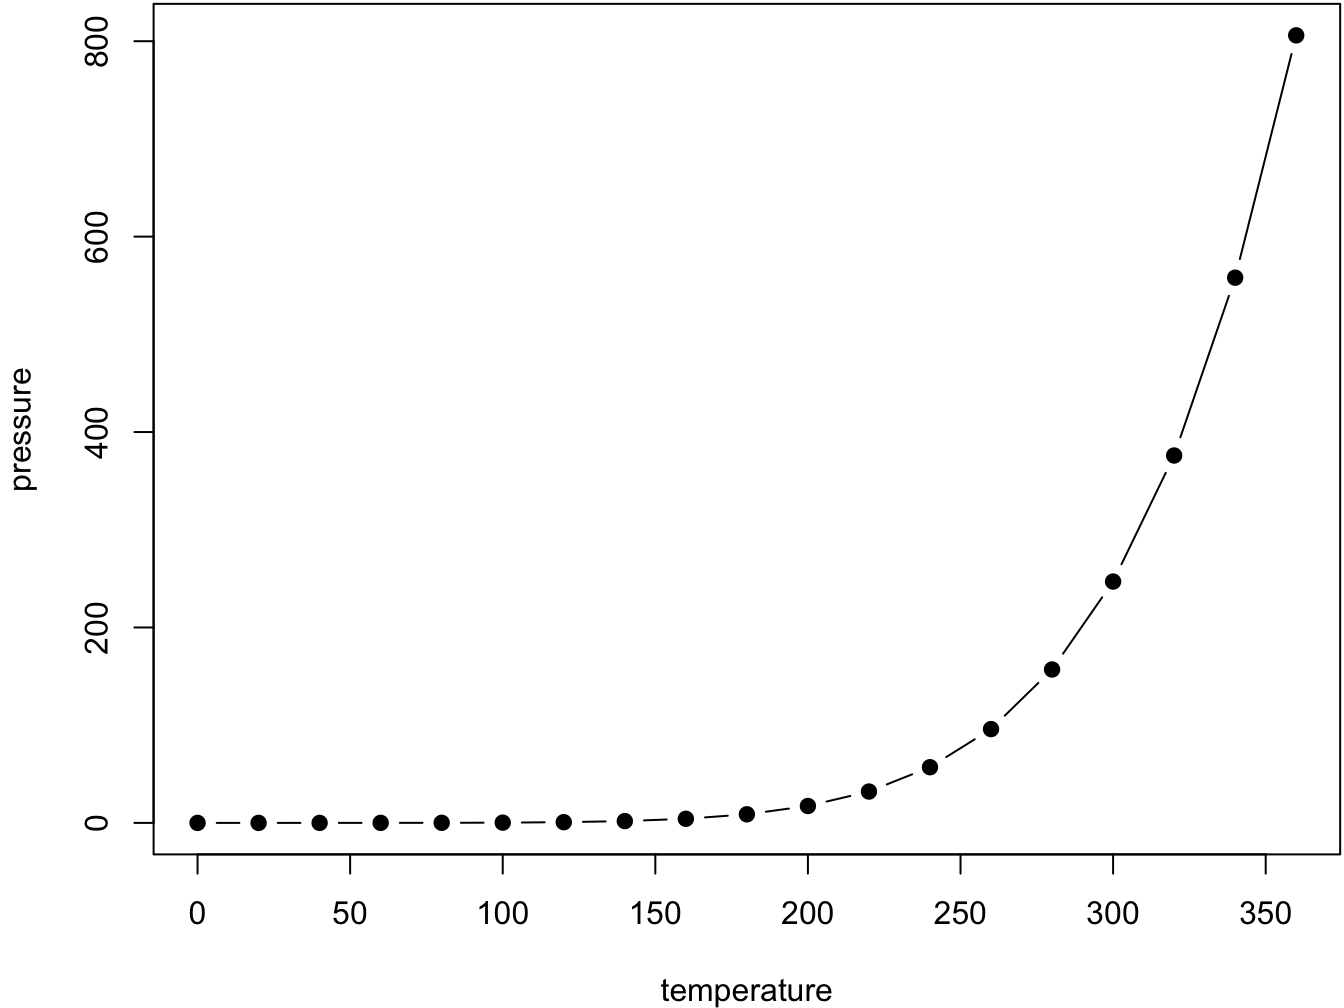
\includegraphics[width=0.8\linewidth]{bookdown-demo_files/figure-latex/nice-fig-1} 

}

\caption{Here is a nice figure!}\label{fig:nice-fig}
\end{figure}

Reference a figure by its code chunk label with the \texttt{fig:} prefix, e.g., see Figure \ref{fig:nice-fig}. Similarly, you can reference tables generated from \texttt{knitr::kable()}, e.g., see Table \ref{tab:nice-tab}.

\begin{Shaded}
\begin{Highlighting}[]
\NormalTok{knitr}\SpecialCharTok{::}\FunctionTok{kable}\NormalTok{(}
  \FunctionTok{head}\NormalTok{(iris, }\DecValTok{20}\NormalTok{), }\AttributeTok{caption =} \StringTok{\textquotesingle{}Here is a nice table!\textquotesingle{}}\NormalTok{,}
  \AttributeTok{booktabs =} \ConstantTok{TRUE}
\NormalTok{)}
\end{Highlighting}
\end{Shaded}

\begin{table}

\caption{\label{tab:nice-tab}Here is a nice table!}
\centering
\begin{tabular}[t]{rrrrl}
\toprule
Sepal.Length & Sepal.Width & Petal.Length & Petal.Width & Species\\
\midrule
5.1 & 3.5 & 1.4 & 0.2 & setosa\\
4.9 & 3.0 & 1.4 & 0.2 & setosa\\
4.7 & 3.2 & 1.3 & 0.2 & setosa\\
4.6 & 3.1 & 1.5 & 0.2 & setosa\\
5.0 & 3.6 & 1.4 & 0.2 & setosa\\
\addlinespace
5.4 & 3.9 & 1.7 & 0.4 & setosa\\
4.6 & 3.4 & 1.4 & 0.3 & setosa\\
5.0 & 3.4 & 1.5 & 0.2 & setosa\\
4.4 & 2.9 & 1.4 & 0.2 & setosa\\
4.9 & 3.1 & 1.5 & 0.1 & setosa\\
\addlinespace
5.4 & 3.7 & 1.5 & 0.2 & setosa\\
4.8 & 3.4 & 1.6 & 0.2 & setosa\\
4.8 & 3.0 & 1.4 & 0.1 & setosa\\
4.3 & 3.0 & 1.1 & 0.1 & setosa\\
5.8 & 4.0 & 1.2 & 0.2 & setosa\\
\addlinespace
5.7 & 4.4 & 1.5 & 0.4 & setosa\\
5.4 & 3.9 & 1.3 & 0.4 & setosa\\
5.1 & 3.5 & 1.4 & 0.3 & setosa\\
5.7 & 3.8 & 1.7 & 0.3 & setosa\\
5.1 & 3.8 & 1.5 & 0.3 & setosa\\
\bottomrule
\end{tabular}
\end{table}

You can write citations, too. For example, we are using the \textbf{bookdown} package \citep{R-bookdown} in this sample book, which was built on top of R Markdown and \textbf{knitr} \citep{xie2015}.

\hypertarget{analysis}{%
\chapter{Analysis}\label{analysis}}

\hypertarget{summary}{%
\chapter{Summary}\label{summary}}

  \bibliography{book.bib,packages.bib}

\end{document}
